
%!TEX root = ../article.tex

% Entry point for sections:
%
% This file specifies the sections and  its respective order in which they must
% be included.

% Article Sections

\section{Deep learning-based method}
\label{sec:Deep learning-based method}

The emerging deep learning algorithms have been introduced into electrical tomography handling the calculation of non-linear problems.
The applications on EIT and ECT have been frequently discussed, while the implementation of DL methods on EMT is relatively scarce.
Despite various modalities are studied in former researches, the essence of non-linear problems to be solved is consistent, which involves the solution of inverse problem and sensor optimization\cite{Smyl2020Optimizing}.
Due to the fact that the physical models of ECT and EIT are identical in form and similar to the simplified EMT model in low conductivity condition \cite{Cao2011Direct}, the DL methods employed for the image reconstruction of various modalities demonstrate the strong interrelation and a wide range of applicable scenario.

In this section, the key points of deep learning methods for ET inverse problem are addressed, with the emphasis on the theoretical basis of image reconstruction, training sample generation, and DL model issues, \emph{i.e}. architecture, objective/loss function and optimization algorithms.
For each point, the representative design and commonness are illustrated, with the analysis of related characteristics.

\subsection{Theoretical basis of image reconstruction}
\label{subsec:Theoretical basis of image reconstruction}

The basic theory of ET image reconstruction can be divided into two categories, sensitivity-based method and physical model-based method.

\begin{table}
\caption{Theoretical basis of DL modeling.}\label{tab:model_basis}
  \centering
  \footnotesize{
  \begin{tabular}{p{2cm}p{2cm}p{3.5cm}}
  \hline
   Basic method & Research & Characteristics\\
  \hline
   Based on sensitivity & J. Zheng, S. Ren et al.\cite{Zheng2018A,Zheng2019ACNN,Zheng2020ADeep,Ren2020ATwo}& Image processing\\
   D-bar&  S. J. Hamilton, Michael Capps et al.\cite{Hamilton2018Deep,Hamilton2019Beltrami,Capps2021Reconstruction}&Insensitive to boundary shape\\
   BESOM & Z. Wei et al. \cite{Wei2019Dominant,Wei2020Induced} &Modelling of EM field\\
   Feature mapping&  K.S. Jin, X. Li et al. \cite{Jin2019A,Zheng2018AnAuto,Gao2019EIT,Li2021Electrical,Li2020One}&Inverse problem solver\\
  \hline
  \end{tabular}}
\end{table}

The sensitivity of ET, for instance, EIT, is defined according to the perturbation theory, which can be expressed as:
\begin{equation}\label{equ:sensi_define}
S(\sigma ) = \frac{{dz (\sigma )}}{{d\sigma }}\left| {_{\sigma  = {\sigma _0}}} \right.
\end{equation}
where $z$ denotes a boundary measurement.

There exist various approaches to calculate the sensitivity matrix corresponding to the electrode array. For instance, it is convenient and frequently adopted to solve the forward problem by finite element method (FEM) to obtain the sensitivity of each measurement channel, which has been reported in the literature \cite{Yin2010Sensitivity}.

The sensitivity model is formulated as:
\begin{equation}\label{equ:sensi_model}
{\Delta \bf{z}} = {\bf{S}} \Delta \sigma
\end{equation}
where $\bf{S}$ is the sensitivity matrix describing the relationship between conductivity difference in ROI and measurement variation. For simplification, $\Delta \bf{z}$ and $\Delta \sigma$ are replaced by $\bf{z}$ and $\sigma$ in the following content.

It is sophisticated to directly calculate the electrical property because of ill-conditioning and under-determined problems of linear equation (\ref{equ:sensi_model}).

One can combine the available prior knowledge of the solution by employing the regularization strategies to elevate the accuracy and stability of the solution.
Generally, the objective function of regularization methods can be expressed as:
\begin{equation}\label{equ:regularization_gen}
\mathop {\min }\limits_\sigma  {\cal{L}_{{\rm{reg}}}}{\rm{ }} = \left\| {{\bf{S}}\sigma  - {\bf{z}}} \right\|_2^2 + \lambda \cal{R}(\sigma )
\end{equation}
where $ \cal{R}(\sigma )$ represents the regularization term which could be ${\ell}_2$-norm, ${\ell}_1$-norm and total variational penalty.

The regularization strategies effectively improve the solution of tomographic inverse problem, which has been described comprehensively in the previous review\cite{Cui2016A}.
Furthermore, the strategies can also enhance the stability of training procedure and generalization ability of DL method, as analyzed in section \ref{subsec:Objective function}.

The physical model of inverse problem aims at inverting the absolute value of electrical properties by the analytical solution of electromagnetic field variables which are calculated from the boundary information.
In this category, the representative computational inversion methods include the D-bar method and bases-expansion subspace optimization method (BE-SOM)\cite{Wei2019Dominant}.
Specifically, the D-bar method solves the D-bar equation (\ref{equ:sol_Schr_A}) regarding the governing Schr$\ddot{o}$dinger equation (\ref{equ:Schr}) using the scattering transform of DN map, meanwhile BE-SOM calculates the induced contrast current (ICC) and contrast electrical field\cite{Wei2020Induced} then solves the contrast conductivity accordingly.

\subsection{The data samples of DL model}
\label{subsec:The data samples of DL model}

The relationships to be modeled by DL are suggested to be divided into three categories,
\begin{enumerate}
  \item the mapping from data, including measurements and related variables, to target images.
  \item the transform from roughly reconstructed images by a conventional method to targets, in which the DL model severs as the post-processing method.
  \item the relations between measurements (and related variables) and electromagnetic field variables which could calculate the electromagnetic properties accurately.
\end{enumerate}

As a data-driven approach, the DL model learns the non-linear mapping from the input to the output variables given the pair-wise data samples.
In the DL scenario, the data samples are usually categorized as the training set, validation set and testing set which are implemented for the training of DL model variables, validation in the training phase and evaluation in the application stage, respectively.

The quality of training samples determines the performance of image reconstruction.
There exist several noticeable merits of samples characterized by the strong and simple correlations between the input and output variables. This could improve the prediction accuracy of DL model and reduce the complexity of model design.

It is straightforward to fit the relationships 1) and 2) as performed by most of the studies, while several groups attended to realize distinctive transform and indicated promising performance.
H. Zhu, J. Sun \emph{et al.} \cite{Zhu2021Deep} investigated the reconstruction accuracy of a certain DL model using various prevailing reconstruction algorithms, including LBP, Caldron, Landweber iteration and iterative Tikhonov methods, and obtained high-resolution images for all implemented algorithms with well-train networks.
J. Zheng and L. Peng\cite{Zheng2020ADeep} focused on the mere non-linear image residual of the linear reconstruction algorithm for ECT.
In an EIT research, Z. Wei and X. Chen \cite{Wei2020Induced} proposed to construct the mapping from the major part of induced contrast current (ICC) and calculated electric field to the higher order of ICC, by directing the training through setting the multi-level labels of cascade CNNs as the higher-order components.
D. Smyl and D. Liu \cite{Smyl2020Optimizing} introduced the MLP to predict the optimized position of EIT electrodes given the specific optimization indices which consist of the ill-conditioning degree of Hessian matrix and residual of reconstruction.

In addition, the discrepancy between the training and test samples should be taken into serious consideration, especially in the application stage.
The prediction accuracy of a well-trained DL model decreases dramatically if the difference of feature variables of input in the latent space increases, which is primarily because of the dissatisfaction of probability identical distribution and constitute a major challenge in the actual applications\cite{Hampe2020Investigating}.

There exist a variety of computational electromagnetic methods that are able to simulate the electromagnetic field generated by ET sensors.
The software EIDORS is available freely for the forward and inverse modeling of EIT in medical and industrial settings, and to share data and promote collaboration between research groups\cite{Gao2019EIT,Smyl2020Optimizing}.
Furthermore, the commercial FEM and BEM software facilitate the simulation to acquire the boundary measurements for any given tested phantom.
The aforementioned software makes it possible to construct the public database of ET image reconstruction\cite{Zheng2018A}, which is significant to contribute to the DL method development and convincing model evaluation in this field.
The prevailing approaches for ET sample generation, summarized in Table \ref{tab:phantom}, show their distinctions regarding the phantom construction.

\begin{table}
\caption{Phantom constructing method for sample acquisition.}\label{tab:phantom}
  \centering
  \footnotesize{
  \begin{tabular}{p{2cm}p{2cm}p{3.5cm}}
  \hline
   Phantom source & Research & Application scope\\
  \hline
   Geometric structure diagram& J. Lei, J. Xiao et al.\cite{Yang2019Big,Lei2020Computational,Xiao2018Deep,Lei2018Deep,Chen2019Electrical,Tian2019Image,Smyl2020Optimizing,Capps2021Reconstruction} & Similar objectives\\
   High resolution image&  K. Lee, S. Ren et al\cite{Ren2020ATwo,Lee2020Electrical}& Specific objectives\\
   Combined simulation& J. Ye, Z. Xia et al.\cite{Ye2020Investigation,Xia2020Generative} &Simulated subject\\
  \hline
  \end{tabular}}
\end{table}


Most of the studies constructed phantoms by adjusting the shape, location and size of geometric structures, \emph{e.g.} circle and ellipse.
Others appended the approximation phantom of actual objectives obtained from other imaging techniques, for instance, CT scans.
A few studies collected the simulation results of transient processes, close to the actual situation, then fed them into the measurement region of EM field in FEM solver\cite{Xia2020Generative}.
The implementation in gas-liquid-solid three-phase flow measurement enhances the model adaptability for various flow regimes.

\subsection{Architecture of model}
\label{subsec:Architecture of model}

The basic architectures include multi-layer perception (MLP) which consists of fully connected neural networks (FCN) and convolution neural networks (CNN).
Both of the architectures are capable of extracting the input feature and approximately fit the relationships given in section \ref{subsec:The data samples of DL model} by adopting the appropriate depth and hyper-parameters of layers. The main distinction of CNN lies in convolution filter which encodes the local structural data, e.g. images and time series, assuming the local data correlations. The CNN model effectively promotes prediction accuracy in a variety of classification and regression tasks related to images, which makes it also applicable for image reconstruction. For more details and characteristics of CNN, readers could refer to Chapter 9 in literature \cite{Goodfellow2016Deep}.

The model architecture for image reconstruction could employ the fully convolution networks and integration of CNN and FCN, \emph{e.g.} LeNet-5\cite{Lecun1998Gradient,Chao2019Image,Guo2019} as shown in Fig \ref{fig:LeNet}.

\begin{figure}[h]
  \centering
  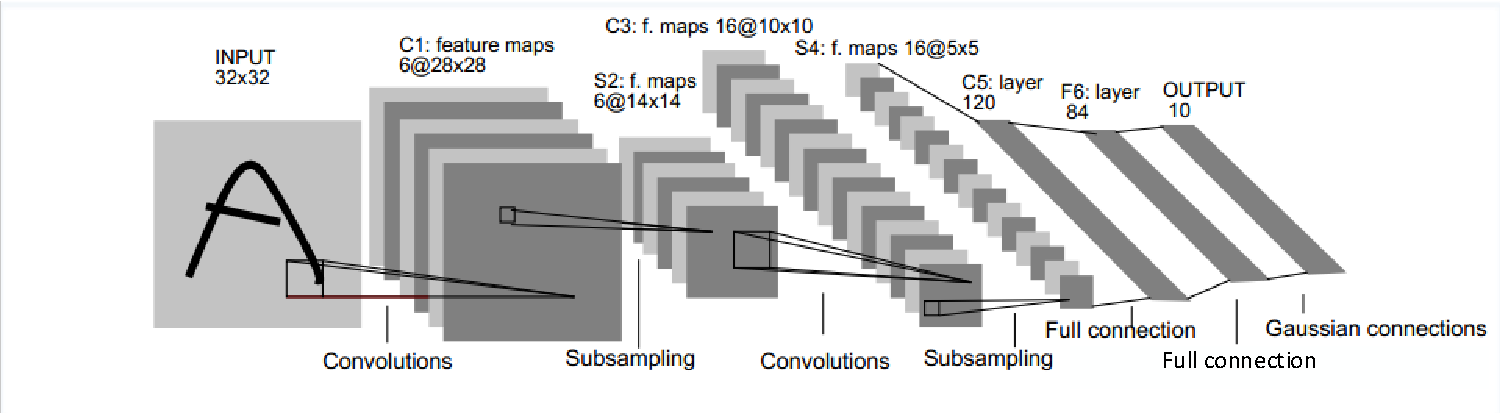
\includegraphics[width=0.99\columnwidth]{figures/LeNet.pdf}
  \caption{Architecture of LeNet-5\cite{Lecun1998Gradient}, the convolution neural networks combining fully connected layers.}\label{fig:LeNet}
\end{figure}

In recent years, full convolution networks have been extensively applied to the image reconstruction problem. The convolution encoder, decoder, as well as combinations and variants of them, were frequently adopted for ET image reconstruction. In U-Net\cite{ronneberger2015unet}, as a classic illustration shown in Fig. \ref{fig:UNet}, the encoder part extracts the low-dimensional features of input variables through the gradual down-sampling and non-linear transform practice, while the decoder reconstructs the target images from the low-dimensional features. There exist skip-connections between encoder and decoder networks, which contribute to utilizing both local and global features for reconstruction in the decoder. The U-Net and other similar convolution auto-encoder architectures have demonstrated the effectiveness regarding the reconstruction utilizing the relationships 1) and 2).

\begin{figure}[h]
  \centering
  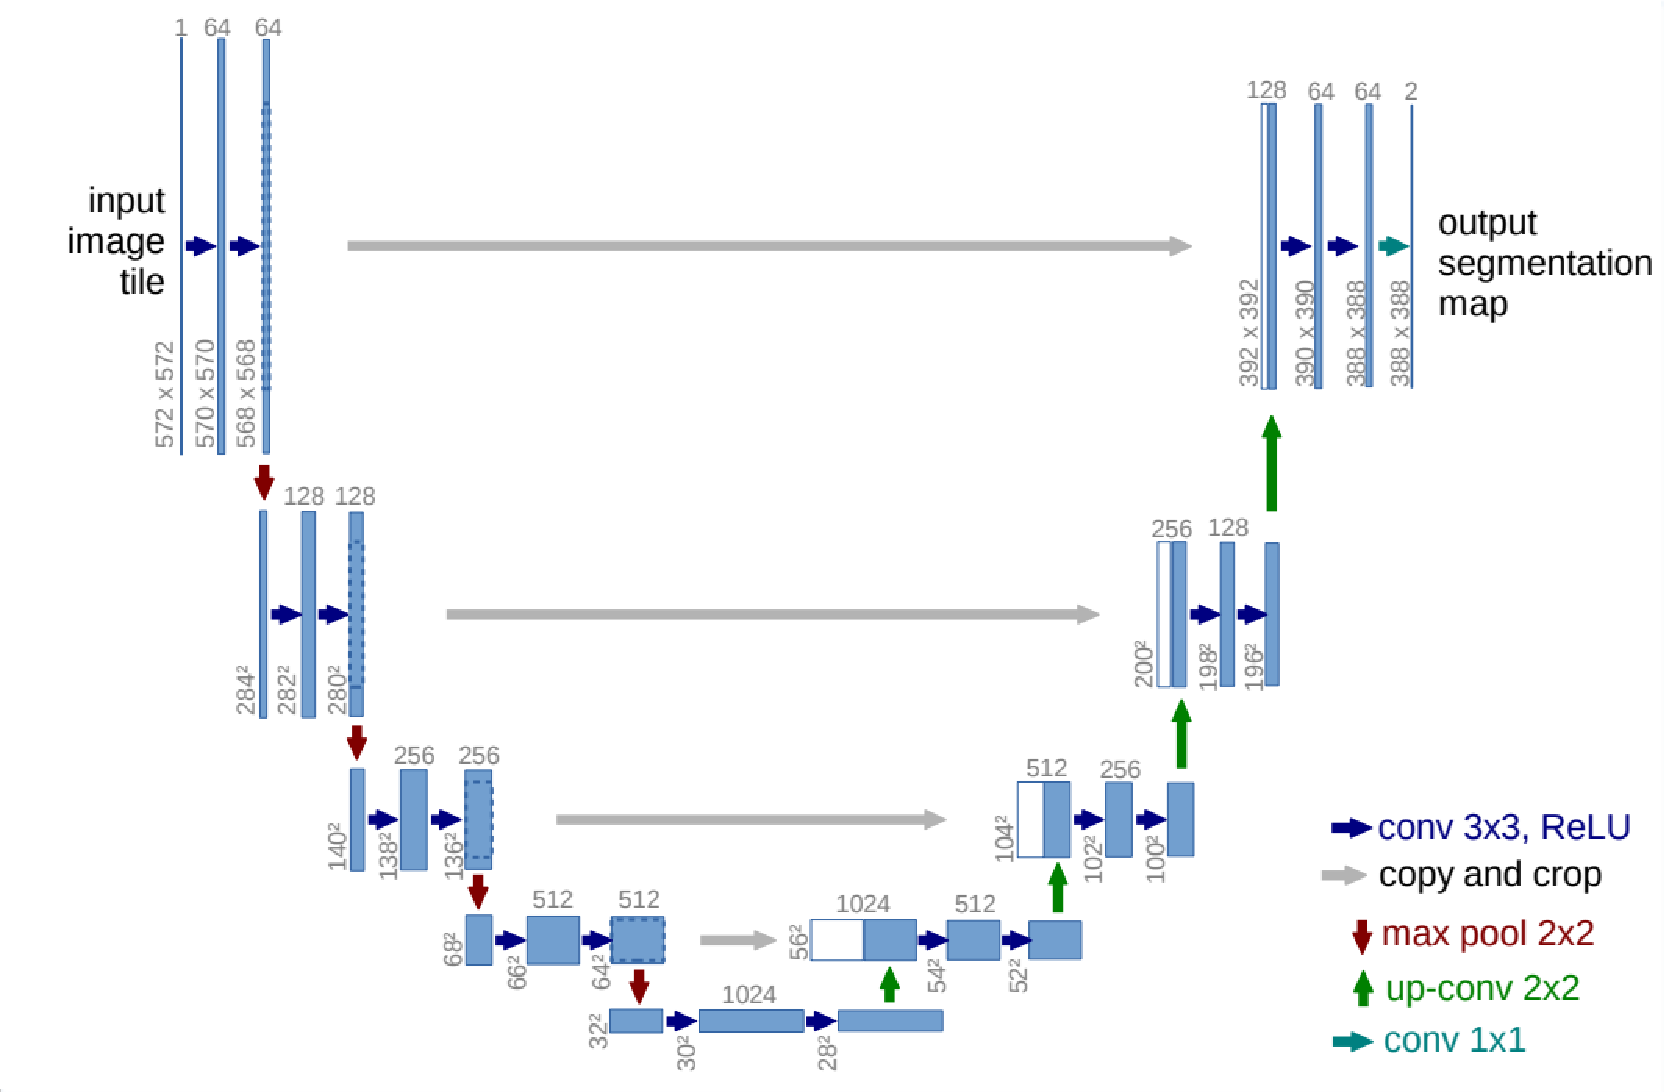
\includegraphics[width=0.99\columnwidth]{figures/UNet.pdf}
  \caption{Architecture of U-Net (example for 32x32 pixels in the lowest resolution)\cite{ronneberger2015unet}}\label{fig:UNet}
\end{figure}

Noted that the forward propagation of input variables in the DL model can be described by the architecture, providing the specific hyper-parameters of layer units which are usually adjusted by empirical and experimental outcomes.

\subsection{Objective function}
\label{subsec:Objective function}

The objective function, also known as the loss function, plays an important role in the training procedure that determines the convergence point and stability of optimization.
Depending on the target of image reconstruction, one should properly design the objective function.

For the reconstruction of EPs with discrete value\cite{Zhu2021Deep,Xiao2018Deep}, \emph{e.g.} binary gray image, the target is essentially a classification task of each image pixel. Usually, the softmax activation function is applied to the output of model and the classification can be achieved by minimizing the cross-entropy loss. For each image pixel, the cross-entropy loss is formulated as:

\begin{equation}\label{equ:crossentropy}
\mathop {\min }\limits_{} {\cal{L}_{{\rm{ce}}}} =  - \sum\limits_{i = 1}^K {{y_i}\log ({{\widehat y}_i})}
\end{equation}
where $K$ is the quantity of gray value categories, $y$ and $\widehat y$ are ground-truth and output of softmax function, respectively.

If the target image is the absolute value of EPs distribution or normalized counterpart, the mean squared error (MSE)\cite{}, mean absolute error (MAE) and smooth $\ell_1$ loss are applicable.
Considering a simple relationship $\widehat y = wx$, $w$ is a trainable parameter which makes $\widehat y $ approximate to $y$, the characteristics of objective functions when $w=1$ are shown in Table \ref{tab:objectives}.
On the one hand, the MSE smoothes the sharp changes or discontinuous region, while the MAE could preserve the inner boundary and address this issue, to some extent.
On the other hand, the gradient of MSE is linearly correlated with error, and that of MAE is constant when the error greater than or less than zero, respectively.
This indicates that the convergence rate of training is quicker by implementing MSE for the gradient descent-based optimization approach.
One could adopt the smooth $\ell_1$ loss which combines the merits of both MAE and MSE.

The regularization over reconstructed image imposes the prior information of EP distribution, achieving the improved spatial resolution clear internal boundaries and reduced artefact. J. Lei \emph{et al.} incorporated the DL model, as a denoiser prior model\cite{Lei2018Deep,Chu2019Prior,Lei2020Computational} compensating the image error caused by the classical algorithms, into the solver which minimizes the objective function for ECT:
\begin{equation}\label{equ:crossentropy}
\min {\cal{L}_{reg}} = \left\| {{\bf{S}}\varepsilon  - {\bf{c}}} \right\|_1^1 + {\lambda _1}\phi (\varepsilon ) + {\lambda _2}\left\| {{\bf{W}}\varepsilon } \right\|_1^1
\end{equation}
where ${\bf{S}} \in {\mathbb{R}^{m \times n}}$ is the sensitivity matrix, $\bf{c}$ is capacitance measurement vector, $\varepsilon$ is a vector of permittivity distribution, $\phi(\cdot)$ denote a image denoiser model, $\bf{W}$ represents the regularization matrix, $\lambda _1$ and $\lambda _2$ are regularization parameters.

In the proposed inverse solver, the DL model only provides the transitional image which is further optimized by minimizing the constrained form of objective (\ref{equ:crossentropy}), by implementing the split Bregman or alternating direction method of multipliers.
\begin{table}
\caption{Characteristics of MAE, MSE and smooth $\ell_1$ loss}\label{tab:objectives}
  \centering
  \footnotesize{
  \begin{tabular}{p{4.7cm}p{1.2cm}p{1.2cm}}
  \hline
   Objective function & Loss value & Derivative \\
  \hline
   ${\cal{L}_{{\rm{MAE}}}} = \left| {\widehat y - y} \right|$
   &\begin{minipage}{0.17\textwidth}
      \includegraphics[width=15mm, height=12mm]{figures/lmae.pdf}
    \end{minipage}& \begin{minipage}{0.17\textwidth}
      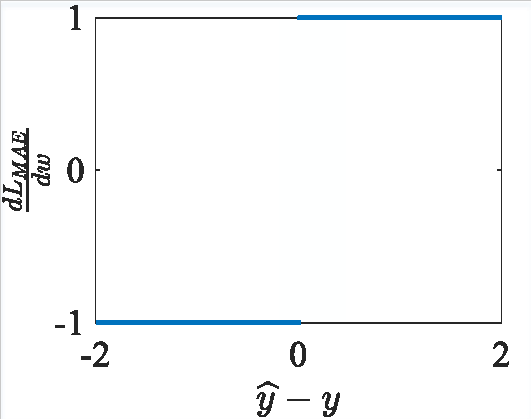
\includegraphics[width=15mm, height=12mm]{figures/dlmae.pdf}
    \end{minipage}\\
   ${\cal{L}_{{\rm{MSE}}}} = {(\widehat y - y)^2}$
   &\begin{minipage}{0.17\textwidth}
      \includegraphics[width=15mm, height=12mm]{figures/lmse.pdf}
    \end{minipage}& \begin{minipage}{0.17\textwidth}
      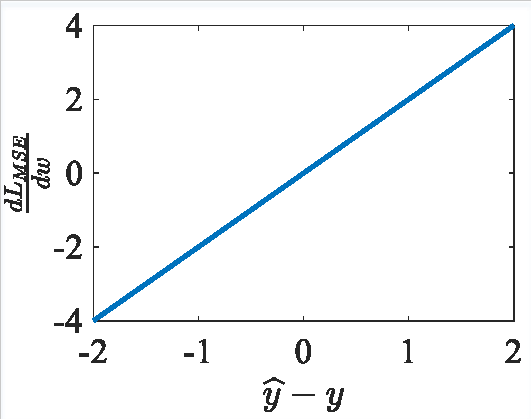
\includegraphics[width=15mm, height=12mm]{figures/dlmse.pdf}
    \end{minipage}\\
   ${\cal{L}_{{\rm{s}}{{\rm{l}}_{\rm{1}}}}} = \left\{ {\begin{array}{*{20}{c}}
{0.5{{(\widehat y - y)}^2}{\rm{ \ \ }}\left| {\widehat y - y} \right| < 1}\\
{\left| {\widehat y - y} \right| - 0.5{\rm{ \ }}otherwise}
\end{array}} \right.$
   &\begin{minipage}{0.17\textwidth}
      \includegraphics[width=15mm, height=12mm]{figures/lsl1.pdf}
    \end{minipage}& \begin{minipage}{0.17\textwidth}
      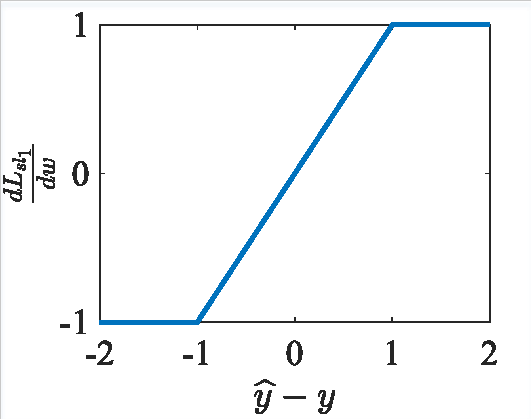
\includegraphics[width=15mm, height=12mm]{figures/dlsl1.pdf}
    \end{minipage}\\
  \hline
  \end{tabular}}
\end{table}

To overcome the over-fitting of model and elevate the generalization ability, the regularization term of weight parameters should be appended in the objective function, including the $\ell_1$-norm and $\ell_2$-norm regularization.
Both of the regularization terms can attenuate the over-fitting by regulating a large number of weight parameters in DL model.
In comparison, the $\ell_1$-norm term shrinkage those weight parameters that contribute less to the error, while $\ell_2$-norm term leads to the sparse weight distribution in each network layer, facilitating the feature selection. The fundamental analysis of regularization term can be found in Chapter 7 of \cite{Goodfellow2016Deep}.

In recent studies, adversarial learning strategies have been introduced into the image reconstruction of ET.
The generative adversarial networks \cite{Goodfellow2014} rely on the adversarial loss during the training procedure, in which the generator and discriminator networks are constructed separately meanwhile trained simultaneously according to the loss function:
\begin{equation}\label{equ:GAN_loss}
\begin{aligned}
\mathop {\min }\limits_G \mathop {\max }\limits_D {\cal{L}_{{\rm{GAN}}}}(D,G) &= {\mathbb{E}_x}_{\sim{p_{{\rm{data}}}}(x)}[\log D(x)] \\ &+
{\mathbb{E}_z}_{\sim{p_z}(z)}[\log (1 - D(g(z))]
\end{aligned}
\end{equation}
where $G$ and $D$ represent the non-linear mapping of generator and discriminator, $x$ and $z$ denote the ideal and generated output variables, of which the probability distributions are $p_{{\rm{data}}}(x)$ and ${p_z}(z)$, respectively.

Minimizing the GAN loss is equivalent to decrease the Jensen–Shannon divergence (JSD) between two distributions, which makes the predicted image more approximate to the real one, in the sense of probability distribution, and looks more realistic.
Nevertheless, the gradient of the objective function (\ref{equ:GAN_loss}) with respect to parameters in the generator would vanish, once the performance of discriminator is much better\cite{arjovskyy2017b}. And the training procedure is usually lacking enough stability.

Accordingly, the improvements on the objective function of GAN have been proposed, by replacing the JSD to be minimized by the Earth-Mover (EM) distance \cite{arjovsky2017}, of which the gradient will not vanish for all parts of probability space. The related loss function is:
\begin{equation}\label{equ:WGAN_loss}
\begin{aligned}
\mathop {\min }\limits_G \mathop {\max }\limits_{\left\| D \right\| < K} {\cal{L}_{{\rm{WGAN}}}}(D,G) &= {\mathbb{E}_x}_{\sim{p_{{\rm{data}}}}(x)}[D(x)] \\ &+
{\mathbb{E}_z}_{\sim{p_z}(z)}[D(g(z))]
\end{aligned}
\end{equation}
where $K$ is a Lipschitz constant.

Furthermore, the objective function (\ref{equ:GAN_loss}) can be changed to a least-squares manner, leading to
\begin{equation}\label{equ:LSGAN_loss}
\left\{
\begin{aligned}
\mathop {\min }\limits_D {\cal{L}_{{\rm{LSGAN}}}}(D) &= {\mathbb{E}_x}_{\sim{p_{{\rm{data}}}}}[{{(D(x) - 1)}^2}] \\ &+ {\mathbb{E}_{z\sim{p_{\rm{z}}}(z)}}[{{(D(G(x)) + 1)}^2}], \\
\mathop {\min }\limits_G {L_{{\rm{LSGAN}}}}(G) &= {\mathbb{E}_{z\sim{p_{\rm{z}}}(z)}}[D{{(G(x))}^2}]
\end{aligned}
\right.
\end{equation}

This is equivalent to minimize the and Pearson $\chi^2$ divergence\cite{Mao2017} between two distributions.

These practices attenuate the instability of GAN training process meanwhile improve the accuracy of generated images \cite{Wang2019x}.

In the application stage, the measured samples and corresponding probability distribution may differ from the counterparts in the training set. Despite the objective function of pair-wise samples can be minimized, the prediction error is yet inevitable.
One could obtain a large number of measured samples without ground-truth of known EPs, and employing the term for semi-supervise learning in the objective function to increase the prediction accuracy.
The graph Laplacian term\cite{Sheikhpour2017Feature,Sheikhpour2020A}, a semi-supervised approach, can be applied to strengthen the feature selection capability through manifold regularization which reducing the feature distance between the samples with and without know EPs. In this way, the predicted images could be closer to the simulated results, thereby maintaining reasonable accuracy.

\subsection{Optimization method}
\label{subsec:Optimization method}

In the training procedure of DL model, the optimization is carried out to minimize the objective function, by adjusting the trainable parameters in every layer which consist of convolution filter and normalization parameters.

Generally, these parameters are updated according to gradient descent-based algorithms. The representative optimizers implemented in ET reconstruction are shown in Table \ref{tab:optimizer}. There exist several widely adopted optimizers with the adjustable learning rate, of which the characteristics are summarized as follows.

\begin{table}
\caption{Optimizers implemented in image reconstruction.}\label{tab:optimizer}
  \centering
  \footnotesize{
  \begin{tabular}{p{2.5cm}p{2cm}p{3cm}}
  \hline
   Optimizer & Research & Adjustment of learning\\
  \hline
   ADAM& J. Zheng and S. J. Hamilton \emph{et al.}\cite{Zheng2020ADeep,Hamilton2018Deep}& Using moment estimation\\
   SGD& F. Li \emph{et al.} \cite{Li2021Electrical}& Manually setting \\
   Conjugate gradient& Smyl Danny and Liu Dong\cite{Smyl2020Optimizing}&In conjugate direction\\
   Adadelta& M. Capps and J. L. Mueller\cite{Capps2021Reconstruction}&Using expectation\\
  \hline
  \end{tabular}}
\end{table}


The training of DL model using the large-scale data set usually adopts the mini-batch strategy where the loss value and gradient of the objective function are evaluated regarding the mini-batch of samples.
The stochastic gradient descent (SGD) method is designed for training regarding batches, while the learning rate should be appropriately adjusted to guarantee the training efficiency.
The improved optimizers, e.g. Adadelta, RMSprop and Adam frequently applied to ET reconstruction, alleviate this issue by introducing the regularizer of learning rate which is adjusted dynamically according to the gradient of sample batch.
In addition, the conjugate gradient algorithm could also accelerate model training, which updates the parameters along the conjugate direction of the gradient of objective function.

In practice, it is recommended to alternate the appropriate optimizer according to the familiarity of model designer, considering the setting of hyper-parameters.


